\documentclass[12pt,a4paper,titlepage]{article}
\usepackage[utf8]{inputenc}
\usepackage[english,russian]{babel}
\usepackage{amsmath}
\usepackage{amsfonts}
\usepackage{amssymb}
\usepackage{mathrsfs}
\usepackage{indentfirst}
\usepackage[hidelinks]{hyperref}
\usepackage[ddmmyyyy]{datetime}
\usepackage{epigraph}   
\usepackage{graphicx}
\graphicspath{{fig/}}
\usepackage[subnum]{cases}
\usepackage[left=3cm,right=2cm,top=2cm,bottom=2cm]{geometry}
\DeclareMathOperator{\Div}{div}
\DeclareMathOperator{\Rot}{rot}
\DeclareMathOperator{\Grad}{grad}
\DeclareMathOperator{\Arsh}{Arsh}
\DeclareMathOperator{\const}{const}
\DeclareMathOperator{\inv}{inv}
\newcommand{\parder}[2]{\dfrac{\partial {#1}}{\partial {#2}}}
\newcommand{\vecmult}[2]{\left[ \vec{{#1}},\vec{{#2}}   \right]}
\newcommand{\abs}[1]{\left| #1  \right|}
\renewcommand{\vec}[1]{\mathbf{#1}}
\renewcommand{\Re}{\operatorname{Re}}
\renewcommand{\Im}{\operatorname{Im}}

\usepackage{bbold}
\usepackage{mathtools}
\DeclarePairedDelimiter\bra{\langle}{\rvert}
\DeclarePairedDelimiter\ket{\lvert}{\rangle}
\DeclarePairedDelimiterX\braket[2]{\langle}{\rangle}{#1 \delimsize\vert #2}

\date{ }
\author{Petrov M. I.}
\title{\textbf{Quantum Optics} \\ lecture course}


\begin{document}

	\maketitle
	\newpage


	\section{Secondary quantization}
	
	\subsection{Introduction}
	
	Second quantization starts with an expansion of a scalar or vector field (or wave functions) in a basis consisting of a complete set of functions. These expansion functions depend on the coordinates of a single particle. The expansion coefficients have been promoted from ordinary numbers to operators, creation and annihilation operators. A creation operator creates a particle in the corresponding basis function and an annihilation operator annihilates a particle in this function.
	
	
	\subsection{System for $\vec{A}$}
	
	Let us write Maxwell equations in vacuum without any charge in the system (in CGS units):
	\begin{numcases}{}
		\Rot \vec{E} = - \frac{1}{c} \parder{\vec{H}}{t},
		\label{eq:M1} \\
		\Rot \vec{H} = \frac{1}{c} \parder{\vec{E}}{t},
		\label{eq:M2} \\
		\Div \vec{E} = 0,
		\label{eq:M3} \\
		\Div \vec{H} = 0.
		\label{eq:M4}
	\end{numcases}
	It's more convenient to work with potentials but not the fields itself. If we know $\vec{A}$ и $\varphi$, we know the field
	\begin{eqnarray}
		\vec{E} &=& - \frac{1}{c} \parder{\vec{A}}{t} - \nabla \varphi, \label{eq:E_field}\\
		\vec{H} &=& \Rot \vec{A}.
	\end{eqnarray}
	It's easy to construct two (generally speaking infinitely many) different potential which can lead to the same EM fields. So we can put one arbitrary condition for $\vec{A}$ and $\varphi$. Let us use Lorentz gauge:
	\begin{equation}
		\Div \vec{A} = 0.
	\end{equation}
	
	Let us obtain an equation for $\vec{A}$. Substitution of field to the \eqref{eq:M2} gives us
	\begin{equation}
		\Rot \Rot \vec{A} = - \frac{1}{c^2} \parder{^2 \vec{A}}{t^2} - \frac{1}{c} \nabla \parder{\varphi}{t}
	\end{equation}
	and since 
	\begin{equation}
		\Rot \Rot \vec{A} = \underbrace{\Grad \Div \vec{A}}_{\hookrightarrow = 0} - \Div \Grad \vec{A} = - \Delta \vec{A}
	\end{equation} 
	then
	\begin{equation}
		\Delta \vec{A} - \frac{1}{c^2} \parder{^2 \vec{A}}{t^2} = \frac{1}{c} \nabla \parder{\varphi}{t}.
		\label{eq:temp1}
	\end{equation}
	If we do $\nabla\cdot$\eqref{eq:E_field} then we get
	\begin{equation}
		\underbrace{\Div \vec{E}}_{\hookrightarrow=0} = - \underbrace{\frac{1}{c} \parder{}{t} \Div \vec{A}}_{\hookrightarrow=0} - \Delta \varphi \quad \to \quad \Delta \varphi = 0 \quad \to \quad \nabla \varphi = 0.
	\end{equation}
	So we have system for $\vec{A}$:
	\begin{equation}
		\begin{cases}
			\Delta \vec{A} - \dfrac{1}{c^2} \parder{^2 \vec{A}}{t^2} = 0, \\ \\
			\Div \vec{A} = 0.
		\end{cases}
	\end{equation}
	\textit{Remark:} in deriving this system we put $\rho = 0$ and $\vec{j} = 0$.
	
	\subsection{Formulation of the problem}
	
	Let us consider a cube with length of the edge $L$ (fig \ref{fig:cube}). Boundary conditions are periodic with the period $L$. System is considered to be conservative.
	
	\begin{figure}
		\centering
		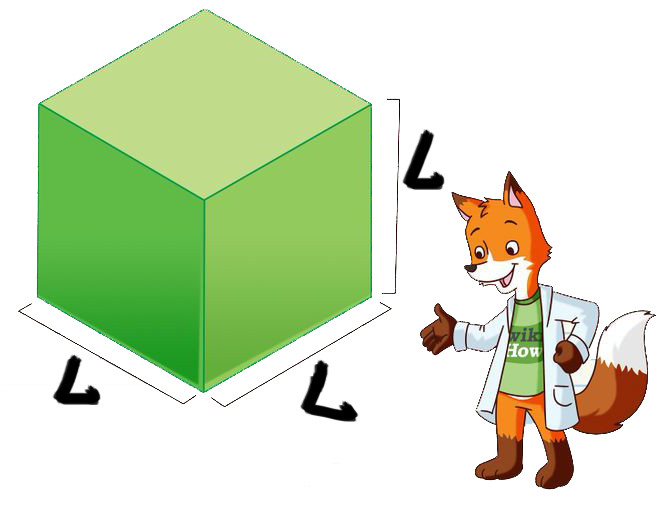
\includegraphics[width=0.5\linewidth]{fig/L1/cube}
		\caption{Formulation of the problem}
		\label{fig:cube}
	\end{figure}

	
\end{document}